% Options for packages loaded elsewhere
\PassOptionsToPackage{unicode}{hyperref}
\PassOptionsToPackage{hyphens}{url}
%
\documentclass[
  ignorenonframetext,
]{beamer}
\usepackage{pgfpages}
\setbeamertemplate{caption}[numbered]
\setbeamertemplate{caption label separator}{: }
\setbeamercolor{caption name}{fg=normal text.fg}
\beamertemplatenavigationsymbolsempty
% Prevent slide breaks in the middle of a paragraph
\widowpenalties 1 10000
\raggedbottom
\setbeamertemplate{part page}{
  \centering
  \begin{beamercolorbox}[sep=16pt,center]{part title}
    \usebeamerfont{part title}\insertpart\par
  \end{beamercolorbox}
}
\setbeamertemplate{section page}{
  \centering
  \begin{beamercolorbox}[sep=12pt,center]{part title}
    \usebeamerfont{section title}\insertsection\par
  \end{beamercolorbox}
}
\setbeamertemplate{subsection page}{
  \centering
  \begin{beamercolorbox}[sep=8pt,center]{part title}
    \usebeamerfont{subsection title}\insertsubsection\par
  \end{beamercolorbox}
}
\AtBeginPart{
  \frame{\partpage}
}
\AtBeginSection{
  \ifbibliography
  \else
    \frame{\sectionpage}
  \fi
}
\AtBeginSubsection{
  \frame{\subsectionpage}
}
\usepackage{amsmath,amssymb}
\usepackage{lmodern}
\usepackage{iftex}
\ifPDFTeX
  \usepackage[T1]{fontenc}
  \usepackage[utf8]{inputenc}
  \usepackage{textcomp} % provide euro and other symbols
\else % if luatex or xetex
  \usepackage{unicode-math}
  \defaultfontfeatures{Scale=MatchLowercase}
  \defaultfontfeatures[\rmfamily]{Ligatures=TeX,Scale=1}
\fi
\usetheme[]{Montpellier}
% Use upquote if available, for straight quotes in verbatim environments
\IfFileExists{upquote.sty}{\usepackage{upquote}}{}
\IfFileExists{microtype.sty}{% use microtype if available
  \usepackage[]{microtype}
  \UseMicrotypeSet[protrusion]{basicmath} % disable protrusion for tt fonts
}{}
\makeatletter
\@ifundefined{KOMAClassName}{% if non-KOMA class
  \IfFileExists{parskip.sty}{%
    \usepackage{parskip}
  }{% else
    \setlength{\parindent}{0pt}
    \setlength{\parskip}{6pt plus 2pt minus 1pt}}
}{% if KOMA class
  \KOMAoptions{parskip=half}}
\makeatother
\usepackage{xcolor}
\IfFileExists{xurl.sty}{\usepackage{xurl}}{} % add URL line breaks if available
\IfFileExists{bookmark.sty}{\usepackage{bookmark}}{\usepackage{hyperref}}
\hypersetup{
  hidelinks,
  pdfcreator={LaTeX via pandoc}}
\urlstyle{same} % disable monospaced font for URLs
\newif\ifbibliography
\usepackage{color}
\usepackage{fancyvrb}
\newcommand{\VerbBar}{|}
\newcommand{\VERB}{\Verb[commandchars=\\\{\}]}
\DefineVerbatimEnvironment{Highlighting}{Verbatim}{commandchars=\\\{\}}
% Add ',fontsize=\small' for more characters per line
\usepackage{framed}
\definecolor{shadecolor}{RGB}{248,248,248}
\newenvironment{Shaded}{\begin{snugshade}}{\end{snugshade}}
\newcommand{\AlertTok}[1]{\textcolor[rgb]{0.94,0.16,0.16}{#1}}
\newcommand{\AnnotationTok}[1]{\textcolor[rgb]{0.56,0.35,0.01}{\textbf{\textit{#1}}}}
\newcommand{\AttributeTok}[1]{\textcolor[rgb]{0.77,0.63,0.00}{#1}}
\newcommand{\BaseNTok}[1]{\textcolor[rgb]{0.00,0.00,0.81}{#1}}
\newcommand{\BuiltInTok}[1]{#1}
\newcommand{\CharTok}[1]{\textcolor[rgb]{0.31,0.60,0.02}{#1}}
\newcommand{\CommentTok}[1]{\textcolor[rgb]{0.56,0.35,0.01}{\textit{#1}}}
\newcommand{\CommentVarTok}[1]{\textcolor[rgb]{0.56,0.35,0.01}{\textbf{\textit{#1}}}}
\newcommand{\ConstantTok}[1]{\textcolor[rgb]{0.00,0.00,0.00}{#1}}
\newcommand{\ControlFlowTok}[1]{\textcolor[rgb]{0.13,0.29,0.53}{\textbf{#1}}}
\newcommand{\DataTypeTok}[1]{\textcolor[rgb]{0.13,0.29,0.53}{#1}}
\newcommand{\DecValTok}[1]{\textcolor[rgb]{0.00,0.00,0.81}{#1}}
\newcommand{\DocumentationTok}[1]{\textcolor[rgb]{0.56,0.35,0.01}{\textbf{\textit{#1}}}}
\newcommand{\ErrorTok}[1]{\textcolor[rgb]{0.64,0.00,0.00}{\textbf{#1}}}
\newcommand{\ExtensionTok}[1]{#1}
\newcommand{\FloatTok}[1]{\textcolor[rgb]{0.00,0.00,0.81}{#1}}
\newcommand{\FunctionTok}[1]{\textcolor[rgb]{0.00,0.00,0.00}{#1}}
\newcommand{\ImportTok}[1]{#1}
\newcommand{\InformationTok}[1]{\textcolor[rgb]{0.56,0.35,0.01}{\textbf{\textit{#1}}}}
\newcommand{\KeywordTok}[1]{\textcolor[rgb]{0.13,0.29,0.53}{\textbf{#1}}}
\newcommand{\NormalTok}[1]{#1}
\newcommand{\OperatorTok}[1]{\textcolor[rgb]{0.81,0.36,0.00}{\textbf{#1}}}
\newcommand{\OtherTok}[1]{\textcolor[rgb]{0.56,0.35,0.01}{#1}}
\newcommand{\PreprocessorTok}[1]{\textcolor[rgb]{0.56,0.35,0.01}{\textit{#1}}}
\newcommand{\RegionMarkerTok}[1]{#1}
\newcommand{\SpecialCharTok}[1]{\textcolor[rgb]{0.00,0.00,0.00}{#1}}
\newcommand{\SpecialStringTok}[1]{\textcolor[rgb]{0.31,0.60,0.02}{#1}}
\newcommand{\StringTok}[1]{\textcolor[rgb]{0.31,0.60,0.02}{#1}}
\newcommand{\VariableTok}[1]{\textcolor[rgb]{0.00,0.00,0.00}{#1}}
\newcommand{\VerbatimStringTok}[1]{\textcolor[rgb]{0.31,0.60,0.02}{#1}}
\newcommand{\WarningTok}[1]{\textcolor[rgb]{0.56,0.35,0.01}{\textbf{\textit{#1}}}}
\setlength{\emergencystretch}{3em} % prevent overfull lines
\providecommand{\tightlist}{%
  \setlength{\itemsep}{0pt}\setlength{\parskip}{0pt}}
\setcounter{secnumdepth}{-\maxdimen} % remove section numbering
%\documentclass[unicode,10pt]{beamer}% 'unicode'が必要
\usepackage{luatexja}% 日本語を使う場合は必須
%\usepackage[japanese]{babel}	
%\usefonttheme[onlymath]{serif}
%\usepackage[T1]{fontenc} %これを使うと、ギリシャ文字が出ない
%\usepackage{textcomp}
%\usepackage[scale=1.0]{tgheros} % Sans serif font
%\usepackage[scaled]{beramono} % Monospace font
%\usepackage{luatexja-otf}
%\renewcommand{\kanjifamilydefault}{\gtdefault}
%\usepackage[haranoaji]{luatexja-preset}

% スライド番号の表示 %%%%%%%%%%%%%%%%%%%
\makeatletter
\setbeamertemplate{footline}{%
  \leavevmode%
  \hbox{%
  \begin{beamercolorbox}[wd=.5\paperwidth,ht=2.25ex,dp=1ex,right]{date in head/foot}%
    \insertframenumber{} \hspace*{2ex} % new version without total frames
  \end{beamercolorbox}}%
  \vskip0pt%
}
\makeatother
% スライド番号の表示 %%%%%%%%%%%%%%%%%%%
\ifLuaTeX
  \usepackage{selnolig}  % disable illegal ligatures
\fi

\title{第4章: 予測}
\subtitle{Elena Llaudet \& Kosuke Imai.\\
Data Analysis for Social Science: A Friendly and Practical
Introduction.}
\author{}
\date{\vspace{-2.5em}2026-03-09}

\begin{document}
\frame{\titlepage}

\hypertarget{ux4e88ux6e2cux3068ux306fux4f55ux304b}{%
\section{4.1
予測とは何か？}\label{ux4e88ux6e2cux3068ux306fux4f55ux304b}}

\begin{frame}{予測の重要性}
\protect\hypertarget{ux4e88ux6e2cux306eux91cdux8981ux6027}{}
\begin{itemize}
\tightlist
\item
  過去のデータを用いて、未知の状況や未来の結果を推測する。
\item
  社会科学における例：

  \begin{itemize}
  \tightlist
  \item
    選挙結果の予測
  \item
    経済指標（GDP成長率など）の予測
  \item
    犯罪率や教育効果の予測
  \end{itemize}
\item
  予測の精度を上げるために、\textbf{線形回帰} (Linear Regression)
  という手法を学ぶ。
\end{itemize}
\end{frame}

\hypertarget{ux6563ux5e03ux56f3ux3068ux7ddaux5f62ux95a2ux4fc2}{%
\section{4.2
散布図と線形関係}\label{ux6563ux5e03ux56f3ux3068ux7ddaux5f62ux95a2ux4fc2}}

\begin{frame}[fragile]{precincts データの読み込み (1)}
\protect\hypertarget{precincts-ux30c7ux30fcux30bfux306eux8aadux307fux8fbcux307f-1}{}
\begin{itemize}
\tightlist
\item
  2019年ウクライナ大統領選挙の投票区レベルデータを読み込みます。
\end{itemize}

\scriptsize

\begin{Shaded}
\begin{Highlighting}[]
\CommentTok{\# 1. ローカルに保存したデータの読み込み（推奨）}
\NormalTok{precincts }\OtherTok{\textless{}{-}} \FunctionTok{read.csv}\NormalTok{(}\StringTok{"UA\_precincts.csv"}\NormalTok{)}

\CommentTok{\# （参考）URLから直接読み込むことも可能}
\CommentTok{\# precincts \textless{}{-} read.csv("https://ayumu{-}tanaka.github.io/QSS/DSS\_Data/UA\_precincts.csv")}
\end{Highlighting}
\end{Shaded}

\normalsize
\end{frame}

\begin{frame}[fragile]{データの確認 (2)}
\protect\hypertarget{ux30c7ux30fcux30bfux306eux78baux8a8d-2}{}
\scriptsize

\begin{Shaded}
\begin{Highlighting}[]
\CommentTok{\# 最初の数行を表示}
\FunctionTok{head}\NormalTok{(precincts)}
\end{Highlighting}
\end{Shaded}

\begin{verbatim}
##   russian_tv pro_russian prior_pro_russian within_25km
## 1          0   2.7210884          25.14286           1
## 2          0   0.8928571          35.34483           0
## 3          1   1.6949153          20.53232           1
## 4          0  72.2689076          84.47761           1
## 5          0   1.2820513          28.99408           0
## 6          1   1.4285714          45.58824           0
\end{verbatim}

\normalsize
\end{frame}

\begin{frame}[fragile]{散布図の作成}
\protect\hypertarget{ux6563ux5e03ux56f3ux306eux4f5cux6210}{}
\begin{itemize}
\tightlist
\item
  2つの数値変数の関係を視覚化する。
\item
  例：過去の親ロシア派への投票率（\texttt{prior\_pro\_russian}）と、今回の親ロシア派への投票率（\texttt{pro\_russian}）。
\end{itemize}
\end{frame}

\begin{frame}[fragile]{散布図のコード}
\protect\hypertarget{ux6563ux5e03ux56f3ux306eux30b3ux30fcux30c9}{}
\begin{Shaded}
\begin{Highlighting}[]
\CommentTok{\# 散布図のプロット}
\FunctionTok{plot}\NormalTok{(precincts}\SpecialCharTok{$}\NormalTok{prior\_pro\_russian, precincts}\SpecialCharTok{$}\NormalTok{pro\_russian,}
     \AttributeTok{xlab =} \StringTok{"Prior Pro{-}Russian Vote (\%)"}\NormalTok{, }
     \AttributeTok{ylab =} \StringTok{"Current Pro{-}Russian Vote (\%)"}\NormalTok{,}
     \AttributeTok{main =} \StringTok{"Prior and Current Vote Shares"}\NormalTok{)}
\end{Highlighting}
\end{Shaded}

\begin{center}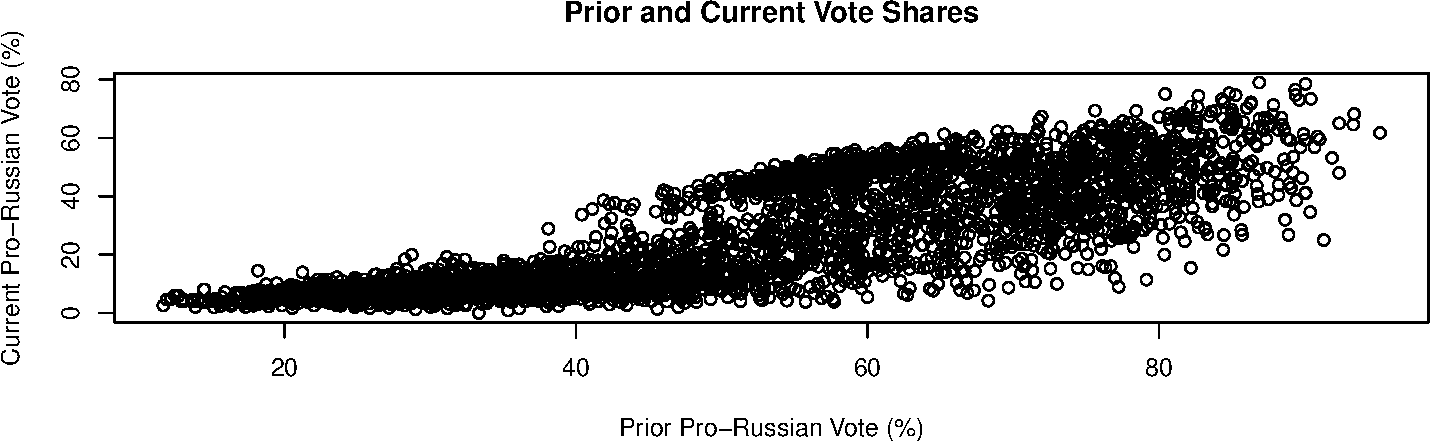
\includegraphics[height=0.4\textheight]{DSS_Ch04_files/figure-beamer/unnamed-chunk-3-1} \end{center}
\end{frame}

\hypertarget{ux7ddaux5f62ux56deux5e30ux30e2ux30c7ux30eb}{%
\section{4.3
線形回帰モデル}\label{ux7ddaux5f62ux56deux5e30ux30e2ux30c7ux30eb}}

\begin{frame}{回帰直線}
\protect\hypertarget{ux56deux5e30ux76f4ux7dda}{}
\begin{itemize}
\tightlist
\item
  散布図の点の間を通る「最もよく当てはまる」直線を引く。
\item
  数式： \(\hat{Y} = \hat{\alpha} + \hat{\beta} X\)

  \begin{itemize}
  \tightlist
  \item
    \(\hat{Y}\): 予測値
  \item
    \(X\): 説明変数（独立変数）
  \item
    \(\hat{\alpha}\): 切片 (Intercept)
  \item
    \(\hat{\beta}\): 傾き (Slope)
  \end{itemize}
\end{itemize}
\end{frame}

\begin{frame}{最小二乗法 (OLS)}
\protect\hypertarget{ux6700ux5c0fux4e8cux4e57ux6cd5-ols}{}
\begin{itemize}
\tightlist
\item
  \textbf{最小二乗法} (Ordinary Least Squares: OLS)
\item
  観測値 \(Y_i\) と予測値 \(\hat{Y}_i\) の差（\textbf{残差},
  Residual）の二乗和を最小にする \(\hat{\alpha}\) と \(\hat{\beta}\)
  を求める。
\end{itemize}
\end{frame}

\hypertarget{rux3067ux306eux56deux5e30ux5206ux6790}{%
\section{4.4
Rでの回帰分析}\label{rux3067ux306eux56deux5e30ux5206ux6790}}

\begin{frame}[fragile]{lm() 関数の使用}
\protect\hypertarget{lm-ux95a2ux6570ux306eux4f7fux7528}{}
\begin{itemize}
\tightlist
\item
  \texttt{lm(従属変数\ \textasciitilde{}\ 説明変数,\ data\ =\ データフレーム)}
\end{itemize}

\footnotesize

\begin{Shaded}
\begin{Highlighting}[]
\CommentTok{\# 回帰モデルの推定}
\NormalTok{model }\OtherTok{\textless{}{-}} \FunctionTok{lm}\NormalTok{(pro\_russian }\SpecialCharTok{\textasciitilde{}}\NormalTok{ prior\_pro\_russian, }\AttributeTok{data =}\NormalTok{ precincts)}
\end{Highlighting}
\end{Shaded}

\normalsize
\end{frame}

\begin{frame}[fragile]{モデルの結果}
\protect\hypertarget{ux30e2ux30c7ux30ebux306eux7d50ux679c}{}
\scriptsize

\begin{Shaded}
\begin{Highlighting}[]
\FunctionTok{summary}\NormalTok{(model)}
\end{Highlighting}
\end{Shaded}

\begin{verbatim}
## 
## Call:
## lm(formula = pro_russian ~ prior_pro_russian, data = precincts)
## 
## Residuals:
##     Min      1Q  Median      3Q     Max 
## -38.202  -7.524  -0.107   7.119  25.247 
## 
## Coefficients:
##                     Estimate Std. Error t value Pr(>|t|)    
## (Intercept)       -14.321933   0.530968  -26.97   <2e-16 ***
## prior_pro_russian   0.796611   0.009651   82.55   <2e-16 ***
## ---
## Signif. codes:  0 '***' 0.001 '**' 0.01 '*' 0.05 '.' 0.1 ' ' 1
## 
## Residual standard error: 11.17 on 3587 degrees of freedom
## Multiple R-squared:  0.6551, Adjusted R-squared:  0.655 
## F-statistic:  6814 on 1 and 3587 DF,  p-value: < 2.2e-16
\end{verbatim}

\normalsize
\end{frame}

\begin{frame}[fragile]{推定値の解釈}
\protect\hypertarget{ux63a8ux5b9aux5024ux306eux89e3ux91c8}{}
\begin{itemize}
\tightlist
\item
  \texttt{(Intercept)} (\(\hat{\alpha}\)):
  説明変数が0のときの期待値（理論値）。
\item
  \texttt{prior\_pro\_russian} (\(\hat{\beta}\)):
  過去の投票率が1\%上がると、今回の投票率が何\%変化するか。
\end{itemize}
\end{frame}

\hypertarget{ux4e88ux6e2cux5024ux306eux7b97ux51fa}{%
\section{4.5 予測値の算出}\label{ux4e88ux6e2cux5024ux306eux7b97ux51fa}}

\begin{frame}[fragile]{予測の実行}
\protect\hypertarget{ux4e88ux6e2cux306eux5b9fux884c}{}
\begin{itemize}
\tightlist
\item
  推定された係数を用いて、特定の過去の投票率（例：60\%）のときの予測値を算出する。
\end{itemize}

\begin{Shaded}
\begin{Highlighting}[]
\CommentTok{\# 係数の取り出し}
\FunctionTok{coef}\NormalTok{(model)}
\end{Highlighting}
\end{Shaded}

\begin{verbatim}
##       (Intercept) prior_pro_russian 
##       -14.3219329         0.7966111
\end{verbatim}

\begin{Shaded}
\begin{Highlighting}[]
\CommentTok{\# 過去の投票率が60\%の場合の予測値}
\CommentTok{\# pro\_russian = alpha + beta * 60}
\SpecialCharTok{{-}}\FloatTok{14.32} \SpecialCharTok{+}\NormalTok{ (}\FloatTok{0.797}\NormalTok{) }\SpecialCharTok{*} \DecValTok{60}
\end{Highlighting}
\end{Shaded}

\begin{verbatim}
## [1] 33.5
\end{verbatim}
\end{frame}

\begin{frame}[fragile]{predict() 関数}
\protect\hypertarget{predict-ux95a2ux6570}{}
\begin{Shaded}
\begin{Highlighting}[]
\CommentTok{\# predict関数を用いた予測}
\NormalTok{new\_data }\OtherTok{\textless{}{-}} \FunctionTok{data.frame}\NormalTok{(}\AttributeTok{prior\_pro\_russian =} \DecValTok{60}\NormalTok{)}
\FunctionTok{predict}\NormalTok{(model, }\AttributeTok{newdata =}\NormalTok{ new\_data)}
\end{Highlighting}
\end{Shaded}

\begin{verbatim}
##        1 
## 33.47473
\end{verbatim}
\end{frame}

\hypertarget{ux30e2ux30c7ux30ebux306eux9069ux5408ux5ea6}{%
\section{4.6
モデルの適合度}\label{ux30e2ux30c7ux30ebux306eux9069ux5408ux5ea6}}

\begin{frame}[fragile]{決定係数 (R-squared)}
\protect\hypertarget{ux6c7aux5b9aux4fc2ux6570-r-squared}{}
\begin{itemize}
\tightlist
\item
  \(R^2\) は、モデルがデータの変動をどれだけ説明できているかを示す。
\item
  0から1の間の値を取り、1に近いほどモデルの当てはまりが良い。
\end{itemize}

\begin{Shaded}
\begin{Highlighting}[]
\CommentTok{\# summaryの結果からR{-}squaredを確認}
\FunctionTok{summary}\NormalTok{(model)}\SpecialCharTok{$}\NormalTok{r.squared}
\end{Highlighting}
\end{Shaded}

\begin{verbatim}
## [1] 0.6551177
\end{verbatim}
\end{frame}

\hypertarget{ux307eux3068ux3081}{%
\section{4.7 まとめ}\label{ux307eux3068ux3081}}

\begin{frame}[fragile]{第4章のまとめ}
\protect\hypertarget{ux7b2c4ux7ae0ux306eux307eux3068ux3081}{}
\begin{itemize}
\tightlist
\item
  線形回帰を用いて、ある変数から別の変数を予測する方法を学んだ。
\item
  最小二乗法 (OLS) の仕組みを理解した。
\item
  Rの \texttt{lm()}
  関数を用いて回帰分析を実行し、その結果（切片、傾き、決定係数）を解釈した。
\item
  \texttt{predict()} 関数を用いて未知のデータの予測値を算出した。
\end{itemize}
\end{frame}

\end{document}
